\documentclass{beamer}
\usetheme{IMM}

\usepackage{pgf,pgfarrows,pgfnodes,pgfautomata,pgfheaps,pgfshade}
\usepackage{amsmath,amssymb}
\usepackage{colortbl}
\usepackage[english]{babel}
\usepackage{booktabs}
\usepackage{slpython}
\usepackage{underscore}
\usepackage{bm}

\author{Luis Pedro Coelho}
\institute{Programming for Scientists}

\graphicspath{{../figures/}{../figures/generated/}{../images/}}

\newcommand*{\code}[1]{\textsl{#1}}
\newcommand*{\Reals}[1]{R}
\newcommand*{\Assign}{\ensuremath{\leftarrow}}
\newcommand{\creditto}[1]{%
\begin{flushright}
(#1)
\end{flushright}%
}

\title[Python I]{Introduction to Python Programming}
\begin{document}

\frame{\maketitle}

\note{
    Goals for this session:

    - Be able to run a program.
    - Be able to run interactively.

    - Rough understanding of name/object concept.
    - Understand control flow.
}

\begin{frame}[fragile]
\frametitle{Python}

Let's digress for a moment discussing the language\ldots
\end{frame}


\begin{frame}[fragile]
\frametitle{Python Language History}

\begin{block}{History}
\begin{itemize}
\item Python was started in the late 80's.
\item It was intended to be both \alert{easy to teach} and \alert{industrial strength}.
\item It is (has always been) open-source.
\item In the last 10 years, it has become one of the most widely used languages (top 10).
\end{itemize}
\end{block}
\end{frame}

\begin{frame}
\frametitle{Popularity}

\centering
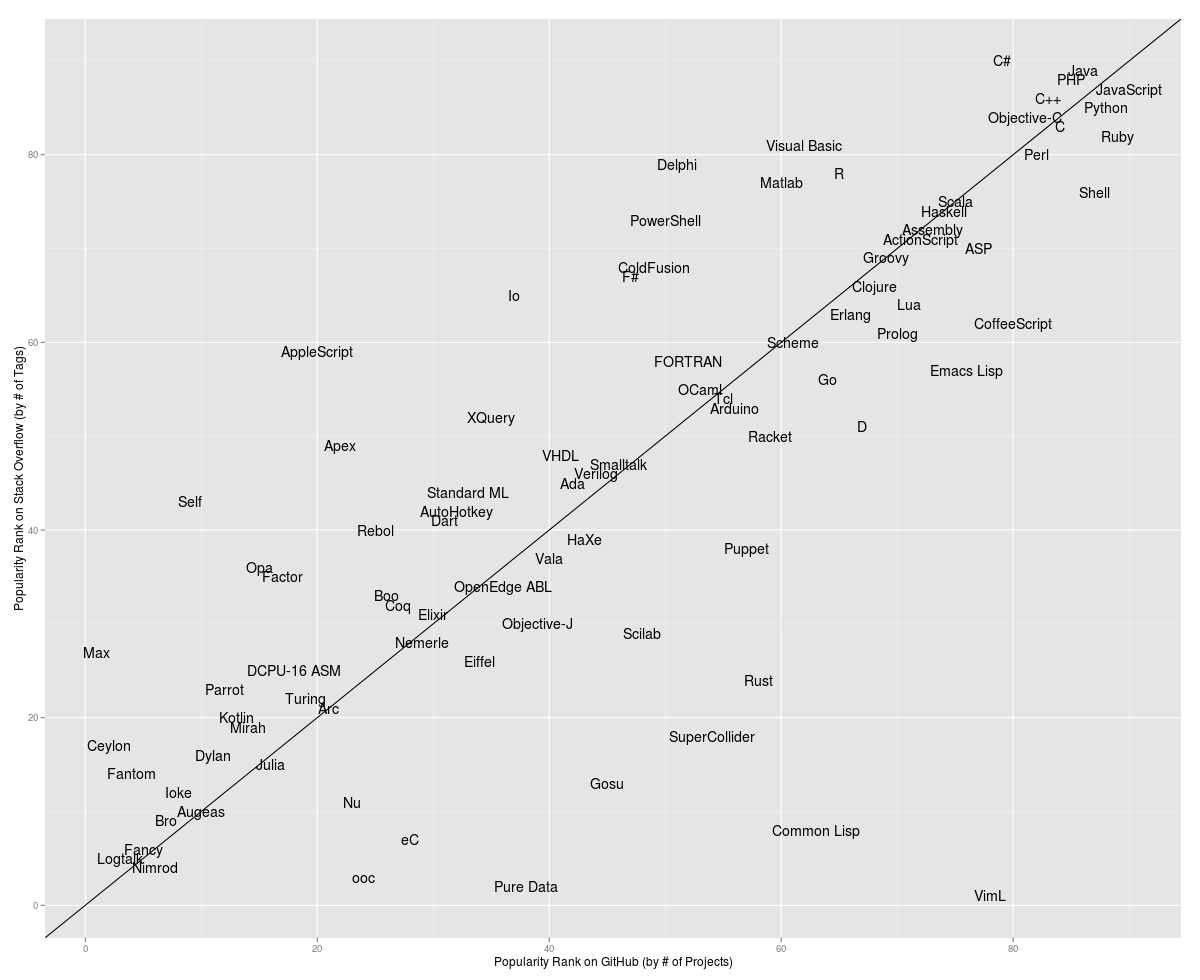
\includegraphics[width=.8\textwidth]{language-ranking-0912.png}

\end{frame}

\begin{frame}
\frametitle{Popularity}

\centering
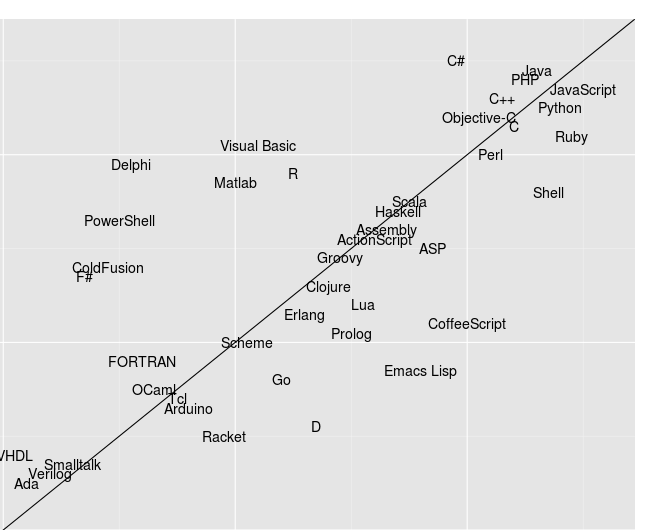
\includegraphics[width=.8\textwidth]{language-ranking-0912-zoom.png}

\end{frame}
\begin{frame}
\frametitle{Python Versions}

\begin{block}{Python Versions}
\begin{itemize}
\item The current versions of Python are \alert{2.7} and \alert{3.3}
\item This class assumes you have 2.6--2.7
\item There are some small differences when compared to version 3.x
\end{itemize}
\end{block}

\end{frame}


\begin{frame}[fragile]
\frametitle{What is a Computer?}

\begin{enumerate}
\item Memory
\item Processor
\item Magic
\end{enumerate}
\end{frame}

\begin{frame}[fragile]
\frametitle{Python Model}

\begin{enumerate}
\item Objects
\item Operations on objects
\item Magic
\end{enumerate}
\end{frame}


\begin{frame}[fragile]
\frametitle{Python Example}

\begin{python}
print "Hello World"
\end{python}
\end{frame}


\begin{frame}[fragile]

\begin{block}{Running Python}
\begin{enumerate}
\item From a file
\item Interactively
\end{enumerate}
\end{block}

\end{frame}

\begin{frame}[fragile]
\frametitle{Computer Program}

\begin{block}{helloword.py}
\begin{python}
print 'Hello World'
\end{python}
\end{block}
\end{frame}

\begin{frame}[fragile]
\frametitle{Running a Program}
\begin{enumerate}
\item Shell
\item IDE
\end{enumerate}
\end{frame}

\begin{frame}[fragile]

\bigskip
\bigskip
\bigskip
Let me show you a demonstration\ldots

\note{
\begin{enumerate}
\item Demo shell with vim
\item Demo one IDE
\end{enumerate}
}


\end{frame}

\begin{frame}[fragile]
\frametitle{More Complex Example}

What is 25 times 5?

\pause
\begin{python}
print 25 * 5
\end{python}
\note{Demo the python shell.

This is basically a glorified calcular}
\end{frame}

\begin{frame}[fragile]
\frametitle{More Complex Example}

\begin{python}
name = 2
other = 3
yetanother = name + other
name = 5
print yetanother + name
\end{python}
\end{frame}

\begin{frame}[fragile]
\frametitle{Blackboard demonstration}

\note{Use the blackboard to introduce the idea of objects, values and names.}
\end{frame}

\begin{frame}[fragile]
\frametitle{Conditionals}

\begin{python}

if <condition>:
    <statement 1>
    <statement 2>
else:
    <statement 3>

\end{python}
\end{frame}

\begin{frame}[fragile]
\frametitle{Lists}

\begin{python}

students = ['Luis','Mark','Rita']

print students[0]
print students[1]
print students[2]
\end{python}

\end{frame}

\begin{frame}[fragile]
\frametitle{Loops}

\begin{python}
students = ['Luis','Mark','Rita',...]

for st in students:
    print st
\end{python}
\end{frame}

\begin{frame}[fragile]
\frametitle{Example}

\begin{python}
values = [0.11, -0.23, -0.16, 0.18, 0.23, 0.19]

sum = 0.0
sum2 = 0.0
for v in values:
    sum = sum + v
    sum2 = sum2 + v * v

mu = sum/len(values)
mu2 = sum2/len(values)
print 'Average: {0}'.format(mu)
print 'Std Dev: {0}'.format(mu2 - mu*mu)
\end{python}
\end{frame}

\begin{frame}[fragile]
\frametitle{Example}

\begin{python}
values = [0.11, -0.23, -0.16, 0.18, 0.23, 0.19]

sum = 0.0
sum2 = 0.0
for v in values:
    sum += v
    sum2 += v * v

mu = sum/len(values)
mu2 = sum2/len(values)
print 'Average: {0}'.format(mu)
print 'Std Dev: {0}'.format(mu2 - mu*mu)
\end{python}
\end{frame}

\begin{frame}[fragile]
\frametitle{Example}

\begin{python}
values = [0.11, -0.23, -0.16, 0.18, 0.23, 0.19]

mu = 0.0
mu2 = 0.0
for v in values:
    mu += v
    mu2 += v * v

mu /= len(values)
mu2 /= len(values)
print 'Average: {0}'.format(mu)
print 'Std Dev: {0}'.format(mu2 - mu*mu)
\end{python}
\end{frame}

\begin{frame}[fragile]
\frametitle{Example}

\begin{python}
values = [0.11, -0.23, -0.16, 0.18, 0.23, 0.19]

mu = 0.0
mu2 = 0.0
for v in values:
    mu += v
    mu2 += v * v

mu /= len(values)
mu2 /= len(values)
print 'Average: {0}'.format(mu)
print 'Std Dev: {0}'.format(mu2 - mu*mu)
\end{python}
\end{frame}

\begin{frame}[fragile]
\frametitle{Exercise}

Adapt the code to ignore negative numbers.

\pause

\begin{python}
values = [0.11, -0.23, -0.16, 0.18, 0.23, 0.19]

mu = 0.0
mu2 = 0.0
n = 0.0
for v in values:
    if v >= 0.0:
        mu += v
        mu2 += v * v
        n += 1

mu /= n
mu2 /= n
print 'Average: {0}'.format(mu)
print 'Std Dev: {0}'.format(mu2 - mu*mu)
\end{python}
\note{
    Negative? strictly negative or just negative.
}

\end{frame}


\begin{frame}[fragile]
\frametitle{Loops (II)}

\begin{block}{Greatest Common Divisor (Euclid's Method)}
\[
gcd(a,b) = \begin{cases}
            a & \text{if $b = a$}\\
            gcd(a-b, b) & \text{if $a > b$} \\
            gcd(a, b-a) & \text{o.w.}
            \end{cases}
\]
\end{block}

\pause
\begin{python}
a = 9344
b = 6497

while a != b:
    if a > b:
        a,b = a-b,b
    else:
        a,b = a,b-a
print a
\end{python}

\end{frame}

\begin{frame}
\frametitle{For Monday}

\begin{itemize}
\item Install Python(x,y)\\
    (or the equivalent on your platform)
\end{itemize}
\end{frame}

\end{document}
